% Editable native annotations around unchanged verified IDE photographs.
\par
\begin{figure}[htbp]
  \centering
  \newsavebox{\MARSrsaproductregistersBox}
  \sbox{\MARSrsaproductregistersBox}{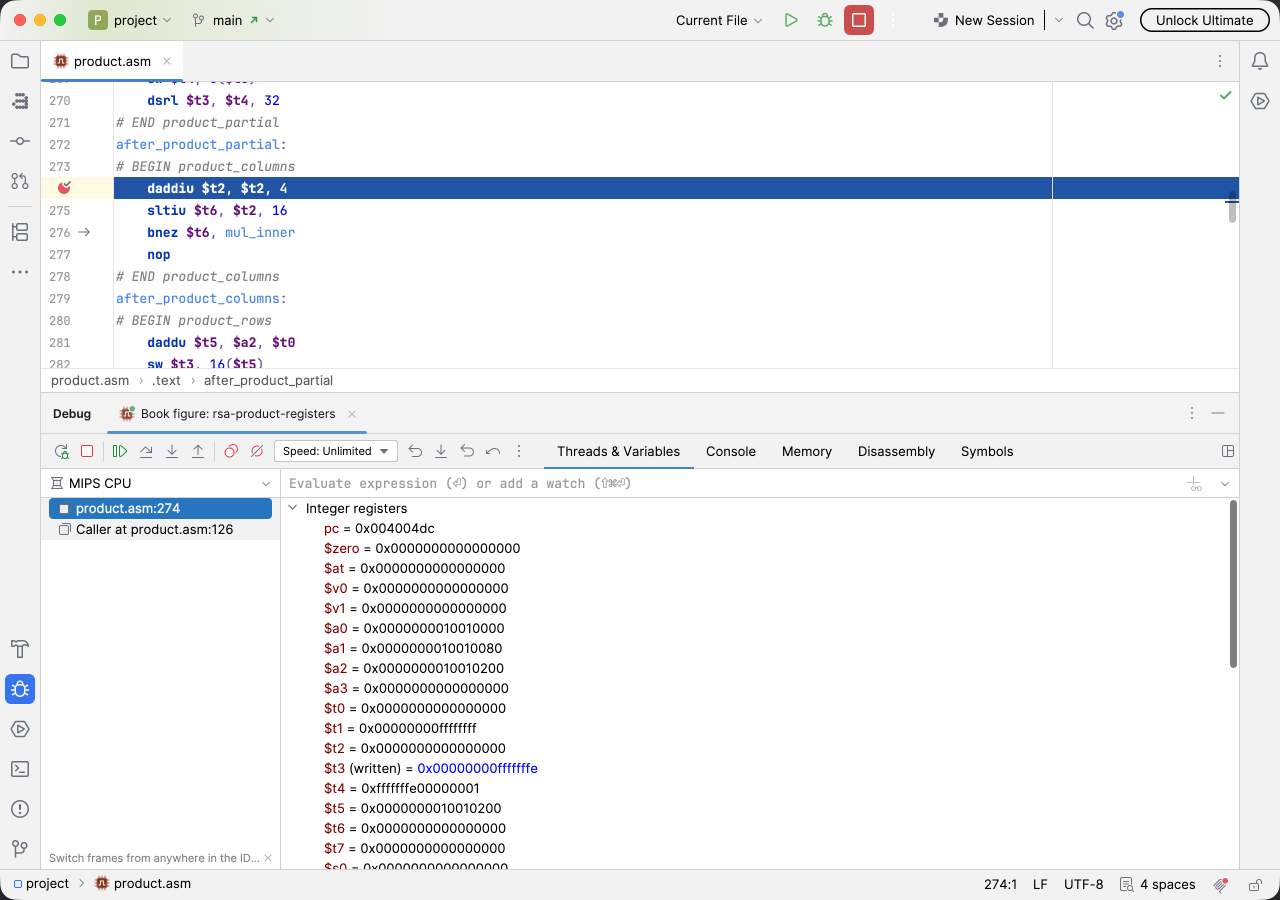
\includegraphics[artifact]{packages/027-rsa-arithmetic/captures/f01/registers.png}}
  \newsavebox{\MARSrsaproductinputsBox}
  \sbox{\MARSrsaproductinputsBox}{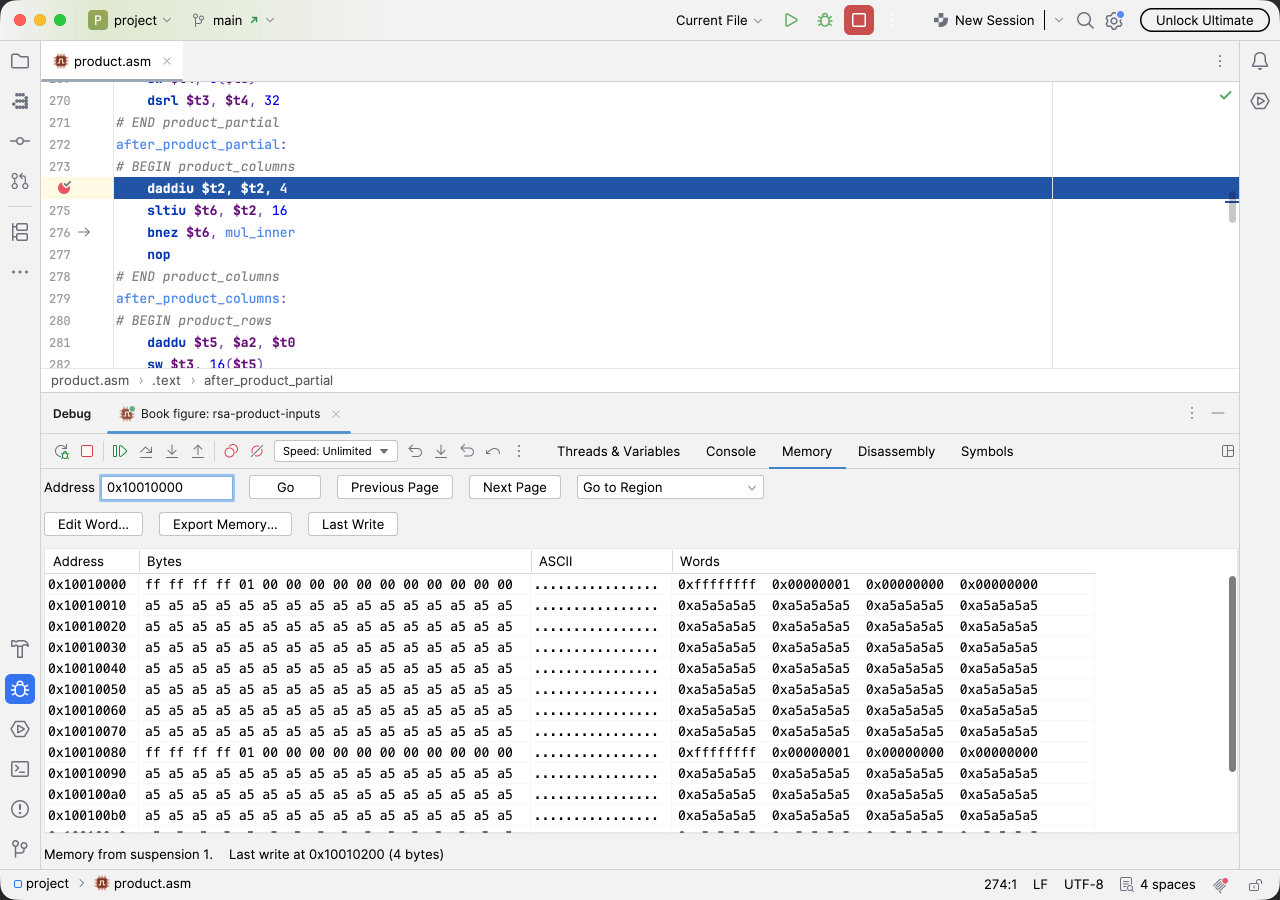
\includegraphics[artifact]{packages/027-rsa-arithmetic/captures/f01/inputs.png}}
  \newsavebox{\MARSrsaproductoutputBox}
  \sbox{\MARSrsaproductoutputBox}{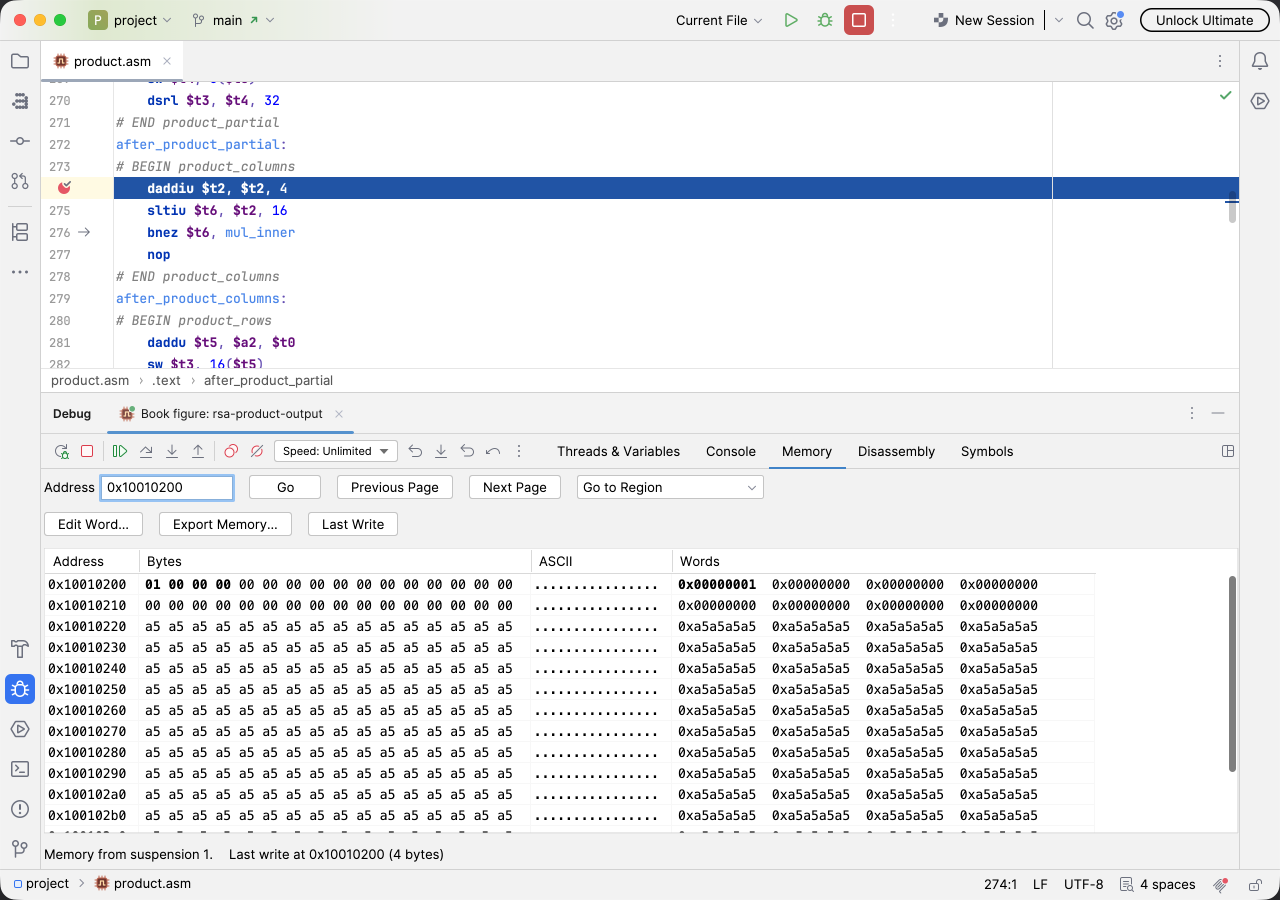
\includegraphics[artifact]{packages/027-rsa-arithmetic/captures/f01/output.png}}
  \edef\MARSrsaproductsourceLeft{\the\dimexpr0.036718750\wd\MARSrsaproductregistersBox\relax}
  \edef\MARSrsaproductsourceBottom{\the\dimexpr0.774444444\ht\MARSrsaproductregistersBox\relax}
  \edef\MARSrsaproductsourceRight{\the\dimexpr0.713281250\wd\MARSrsaproductregistersBox\relax}
  \edef\MARSrsaproductsourceTop{\the\dimexpr0.170000000\ht\MARSrsaproductregistersBox\relax}
  \edef\MARSrsaproductreturnsLeft{\the\dimexpr0.246093750\wd\MARSrsaproductregistersBox\relax}
  \edef\MARSrsaproductreturnsBottom{\the\dimexpr0.112222222\ht\MARSrsaproductregistersBox\relax}
  \edef\MARSrsaproductreturnsRight{\the\dimexpr0.553906250\wd\MARSrsaproductregistersBox\relax}
  \edef\MARSrsaproductreturnsTop{\the\dimexpr0.840000000\ht\MARSrsaproductregistersBox\relax}
  \edef\MARSrsaproductleftLeft{\the\dimexpr0.034375000\wd\MARSrsaproductinputsBox\relax}
  \edef\MARSrsaproductleftBottom{\the\dimexpr0.334444444\ht\MARSrsaproductinputsBox\relax}
  \edef\MARSrsaproductleftRight{\the\dimexpr0.584375000\wd\MARSrsaproductinputsBox\relax}
  \edef\MARSrsaproductleftTop{\the\dimexpr0.608888889\ht\MARSrsaproductinputsBox\relax}
  \edef\MARSrsaproductrightLeft{\the\dimexpr0.034375000\wd\MARSrsaproductinputsBox\relax}
  \edef\MARSrsaproductrightBottom{\the\dimexpr0.147777778\ht\MARSrsaproductinputsBox\relax}
  \edef\MARSrsaproductrightRight{\the\dimexpr0.584375000\wd\MARSrsaproductinputsBox\relax}
  \edef\MARSrsaproductrightTop{\the\dimexpr0.795555556\ht\MARSrsaproductinputsBox\relax}
  \edef\MARSrsaproductoutputLeft{\the\dimexpr0.034375000\wd\MARSrsaproductoutputBox\relax}
  \edef\MARSrsaproductoutputBottom{\the\dimexpr0.311111111\ht\MARSrsaproductoutputBox\relax}
  \edef\MARSrsaproductoutputRight{\the\dimexpr0.584375000\wd\MARSrsaproductoutputBox\relax}
  \edef\MARSrsaproductoutputTop{\the\dimexpr0.608888889\ht\MARSrsaproductoutputBox\relax}
  \begin{tikzpicture}[alt={Five annotated details at the first after_product_partial show accumulator fffffffe00000001 and outgoing carry fffffffe. Each input starts with limbs ffffffff and 00000001. The first stored product limb is one; the seven later limbs remain zero after clearing.}]
    \node[anchor=north west,inner sep=0,font=\small\bfseries] (source-title) at (6mm,0) {Next product instruction};
    \node[anchor=north west,inner sep=0] (source) at ([yshift=-1mm]source-title.south west) {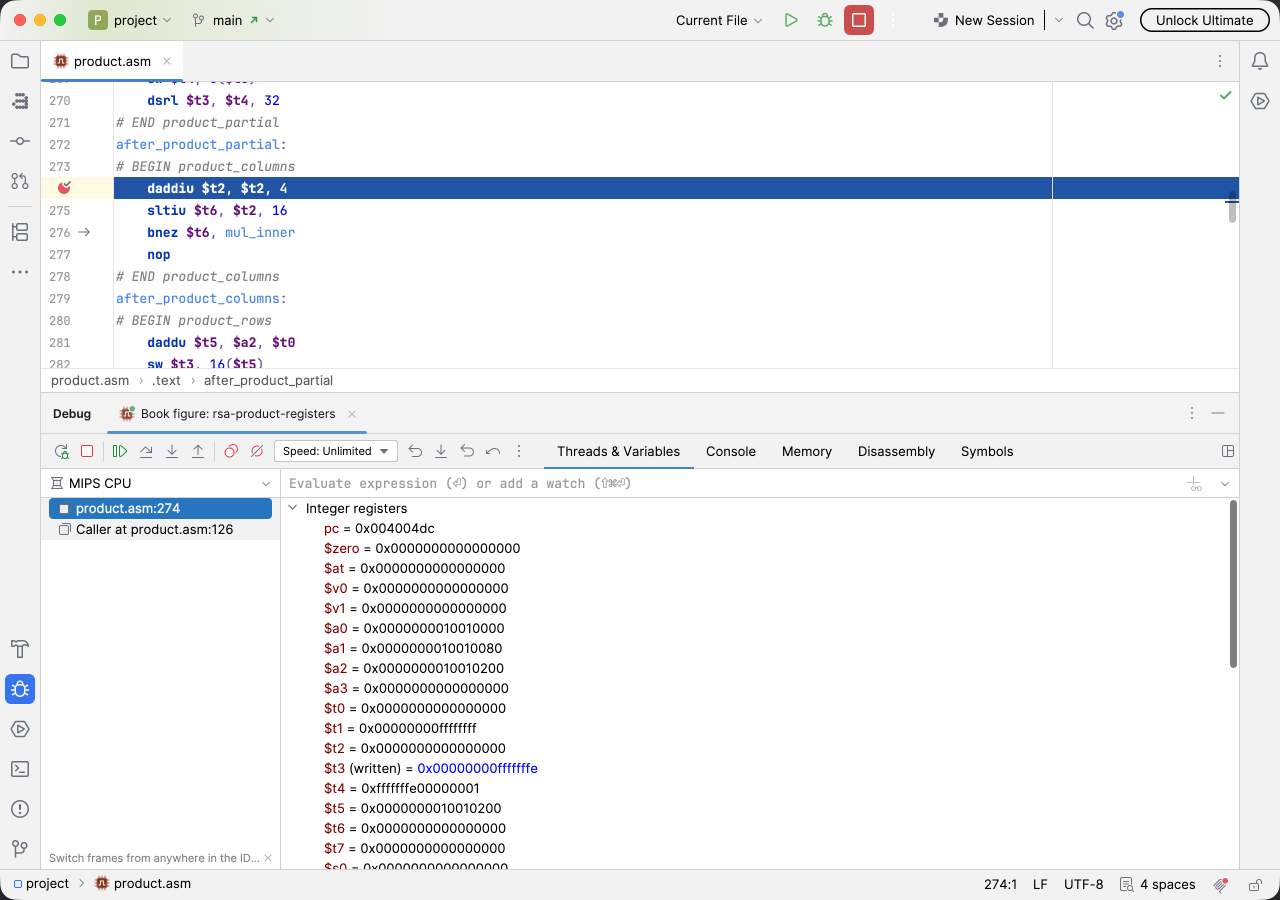
\includegraphics[width=0.54\linewidth,artifact,trim={\MARSrsaproductsourceLeft{} \MARSrsaproductsourceBottom{} \MARSrsaproductsourceRight{} \MARSrsaproductsourceTop{}},clip]{packages/027-rsa-arithmetic/captures/f01/registers.png}};
    \begin{scope}[shift={(source.south west)},x={($(source.south east)-(source.south west)$)},y={($(source.north west)-(source.south west)$)}]
      \draw[black,line width=0.7pt] (0.215625000,0.080000000) rectangle (0.750000000,0.520000000);
      \node[draw=black,fill=white,circle,inner sep=1.5pt,font=\footnotesize] at ($(0.215625000,0.520000000)+(-3mm,0)$) {1};
    \end{scope}
    \node[anchor=north west,inner sep=0,font=\small\bfseries] (returns-title) at ([yshift=-1mm]source.south west) {Carry and full accumulator};
    \node[anchor=north west,inner sep=0] (returns) at ([yshift=-1mm]returns-title.south west) {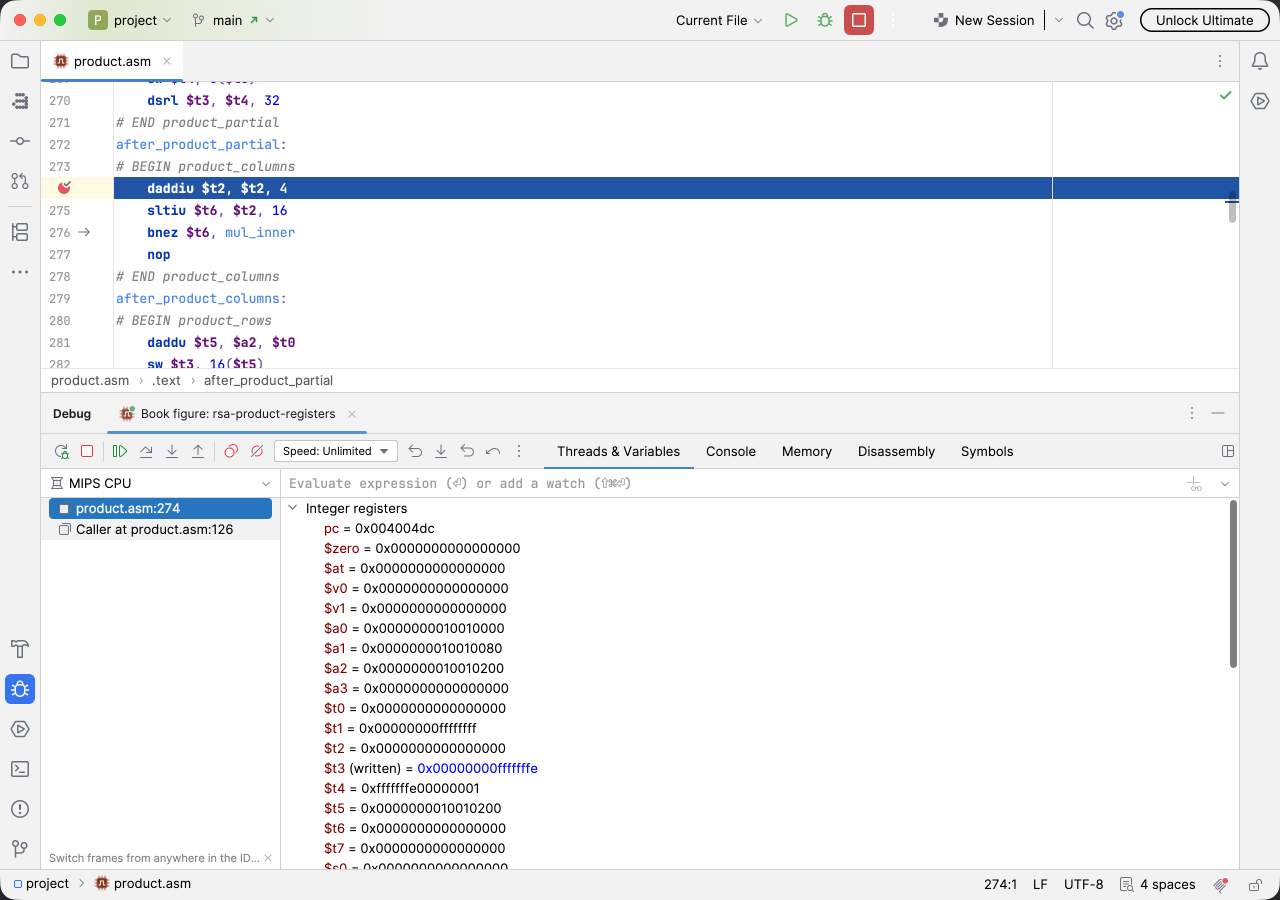
\includegraphics[width=0.52\linewidth,artifact,trim={\MARSrsaproductreturnsLeft{} \MARSrsaproductreturnsBottom{} \MARSrsaproductreturnsRight{} \MARSrsaproductreturnsTop{}},clip]{packages/027-rsa-arithmetic/captures/f01/registers.png}};
    \begin{scope}[shift={(returns.south west)},x={($(returns.south east)-(returns.south west)$)},y={($(returns.north west)-(returns.south west)$)}]
      \draw[black,line width=0.7pt] (0.023437500,0.023255814) rectangle (0.875000000,0.953488372);
      \node[draw=black,fill=white,circle,inner sep=1.5pt,font=\footnotesize] at ($(0.023437500,0.953488372)+(-3mm,0)$) {2};
    \end{scope}
    \node[anchor=north west,inner sep=0,font=\small\bfseries] (left-title) at ([yshift=-1mm]returns.south west) {Left input limbs};
    \node[anchor=north west,inner sep=0] (left) at ([yshift=-1mm]left-title.south west) {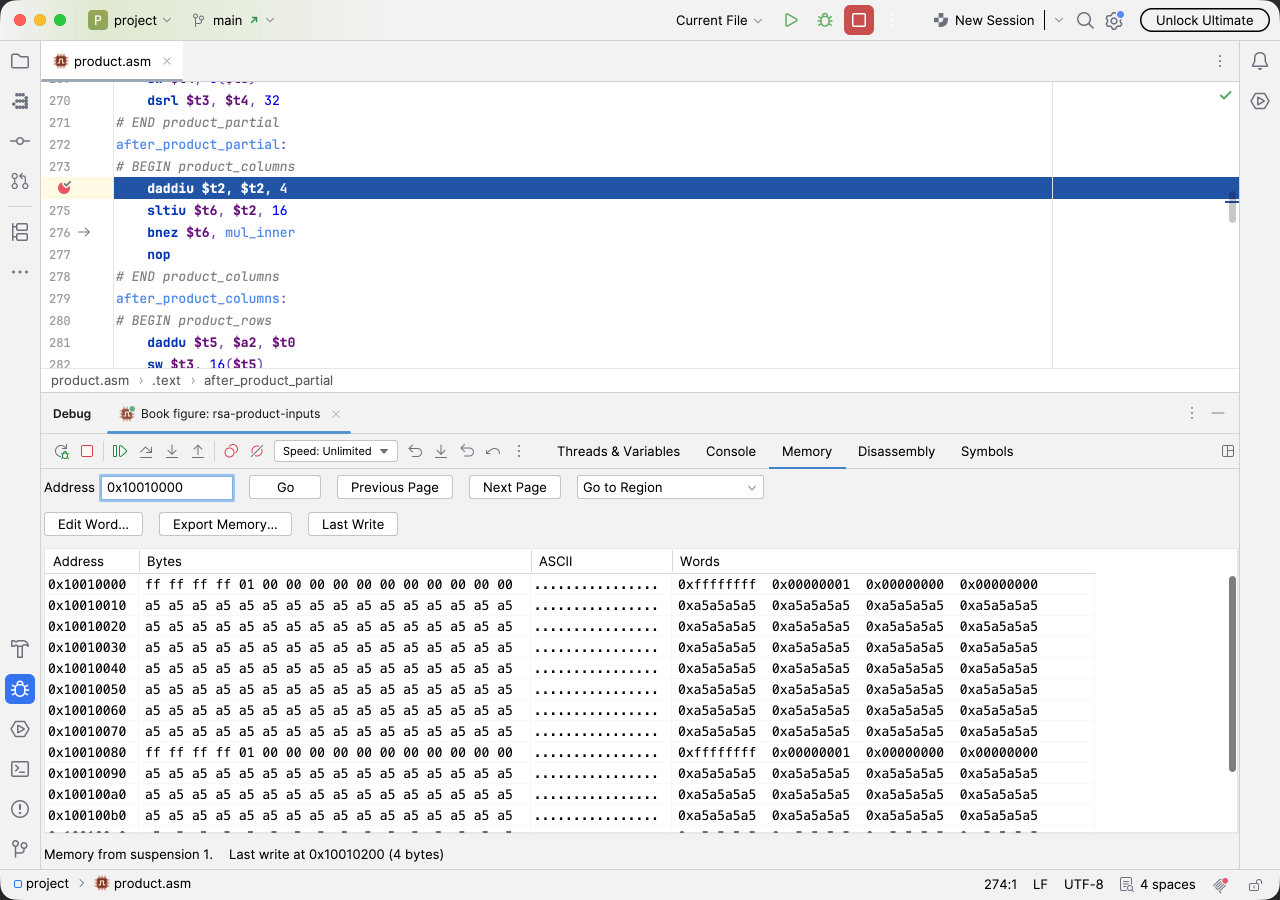
\includegraphics[width=0.84\linewidth,artifact,trim={\MARSrsaproductleftLeft{} \MARSrsaproductleftBottom{} \MARSrsaproductleftRight{} \MARSrsaproductleftTop{}},clip]{packages/027-rsa-arithmetic/captures/f01/inputs.png}};
    \begin{scope}[shift={(left.south west)},x={($(left.south east)-(left.south west)$)},y={($(left.north west)-(left.south west)$)}]
      \draw[black,line width=0.7pt] (0.194672131,0.078431373) rectangle (0.997950820,0.490196078);
      \node[draw=black,fill=white,circle,inner sep=1.5pt,font=\footnotesize] at ($(0,0.490196078)+(-3mm,0)$) {3};
    \end{scope}
    \node[anchor=north west,inner sep=0,font=\small\bfseries] (right-title) at ([yshift=-1mm]left.south west) {Right input limbs};
    \node[anchor=north west,inner sep=0] (right) at ([yshift=-1mm]right-title.south west) {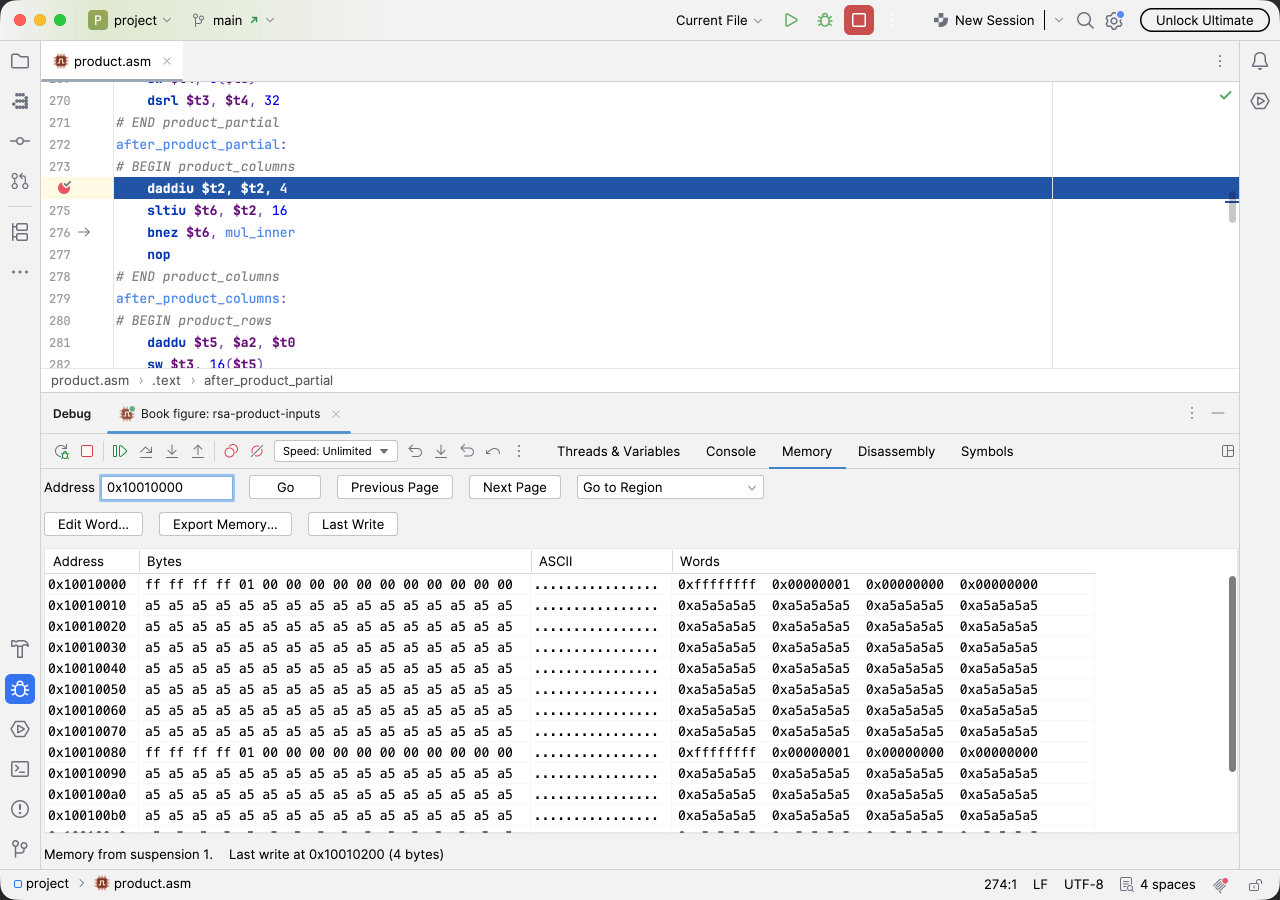
\includegraphics[width=0.84\linewidth,artifact,trim={\MARSrsaproductrightLeft{} \MARSrsaproductrightBottom{} \MARSrsaproductrightRight{} \MARSrsaproductrightTop{}},clip]{packages/027-rsa-arithmetic/captures/f01/inputs.png}};
    \begin{scope}[shift={(right.south west)},x={($(right.south east)-(right.south west)$)},y={($(right.north west)-(right.south west)$)}]
      \draw[black,line width=0.7pt] (0.194672131,0.078431373) rectangle (0.997950820,0.490196078);
      \node[draw=black,fill=white,circle,inner sep=1.5pt,font=\footnotesize] at ($(0,0.490196078)+(-3mm,0)$) {4};
    \end{scope}
    \node[anchor=north west,inner sep=0,font=\small\bfseries] (output-title) at ([yshift=-1mm]right.south west) {First limb and unprocessed product columns};
    \node[anchor=north west,inner sep=0] (output) at ([yshift=-1mm]output-title.south west) {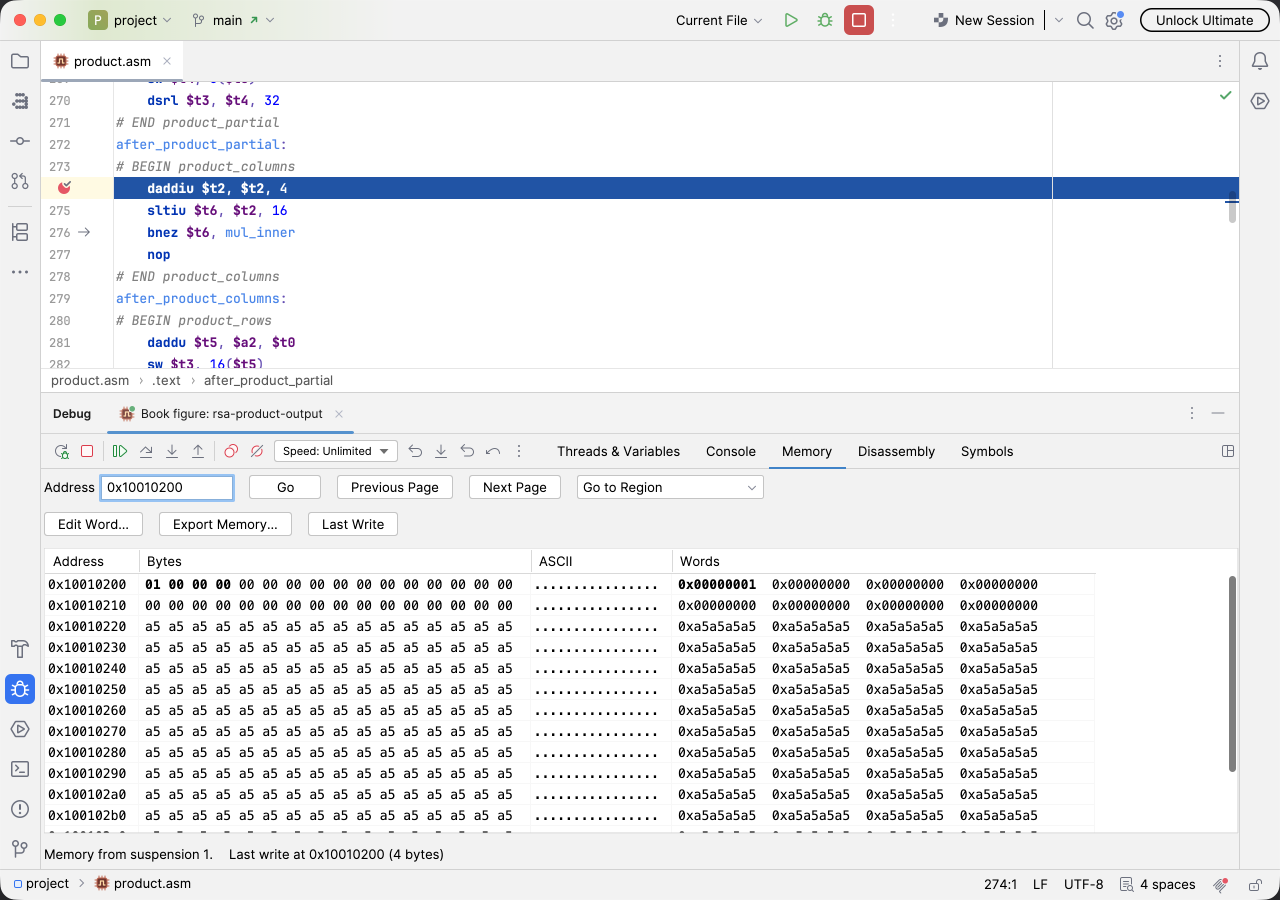
\includegraphics[width=0.84\linewidth,artifact,trim={\MARSrsaproductoutputLeft{} \MARSrsaproductoutputBottom{} \MARSrsaproductoutputRight{} \MARSrsaproductoutputTop{}},clip]{packages/027-rsa-arithmetic/captures/f01/output.png}};
    \begin{scope}[shift={(output.south west)},x={($(output.south east)-(output.south west)$)},y={($(output.north west)-(output.south west)$)}]
      \draw[black,line width=0.7pt] (0.194672131,0.055555556) rectangle (0.997950820,0.638888889);
      \node[draw=black,fill=white,circle,inner sep=1.5pt,font=\footnotesize] at ($(0,0.638888889)+(-3mm,0)$) {5};
    \end{scope}
  \end{tikzpicture}
  \par\smallskip
  \begin{minipage}{\linewidth}
    \small
    \begin{enumerate}
      \setlength{\itemsep}{0pt}
            \setlength{\parsep}{0pt}
      \item This is the first \texttt{after\_product\_partial} visit. One inner product column has been stored; the column walker has not advanced.
      \item \texttt{t4 = 0xfffffffe00000001} is the full 64-bit accumulator. Its low thirty-two bits are the stored limb; \texttt{t3 = 0xfffffffe} carries the upper thirty-two bits to the next column. A word-sized multiply would discard that carry.
      \item The left input begins \texttt{ff ff ff ff 01 00 00 00}: low limbs \texttt{ffffffff} and \texttt{00000001}. Together they represent $2^{33}-1$, not a signed negative integer.
      \item The right input has the same four-limb value. The first column therefore multiplies two \texttt{ffffffff} limbs; later columns must also include both higher input limbs.
      \item The first output word is \texttt{01 00 00 00}. The remaining seven words are still zero from the initial clear. The carry is in a register, so this partial memory image is not yet the complete product.
    \end{enumerate}
  \end{minipage}
  \caption{One product column splits a full accumulator into a limb and a carry.}
  \label{capture:027-rsa-arithmetic-f01}
  \label{rsa-f01}
\end{figure}
\par
